\documentclass[aspectratio=169]{beamer}
\usetheme[block=fill]{metropolis}
\usepackage{tikz}
\usetikzlibrary{shapes.geometric, arrows.meta, positioning, calc}

\title{Building a Reproducible Scholarly Search Toolkit}
\subtitle{Episode 13: Ingesting OpenAlex at Scale}
\author{Scholar Search Kit}
\date{}

\begin{document}

\begin{frame}[plain]
  \titlepage
\end{frame}

\begin{frame}{Episode Goal}
  \begin{alertblock}{The Goal}
    Implement the \texttt{OpenAlexProvider} to securely and politely pull thousands of records from the OpenAlex REST API.
  \end{alertblock}
  \vspace{0.5cm}
  OpenAlex is completely free, but it requires entering the "Polite Pool" via an email header, and limits queries to 100,000 results via Cursor Pagination.
\end{frame}

\begin{frame}{Cursor Pagination}
  \begin{center}
  \resizebox{0.75\linewidth}{!}{
  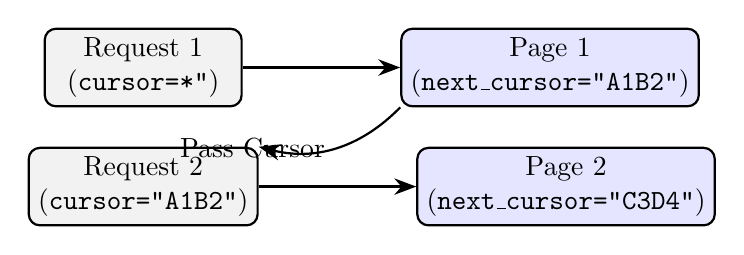
\begin{tikzpicture}[
      node distance=1.5cm and 2cm,
      req/.style={rectangle, draw, thick, rounded corners, minimum width=2.5cm, align=center, fill=black!5},
      resp/.style={rectangle, draw, thick, rounded corners, minimum width=3cm, align=center, fill=blue!10},
      arrow/.style={-{Stealth[scale=1.2]}, thick}
    ]
    
    \node[req] (r1) {Request 1\\(\texttt{cursor=*"})};
    \node[resp, right=of r1] (resp1) {Page 1\\(\texttt{next\_cursor="A1B2"})};
    
    \node[req, below=0.5cm of r1] (r2) {Request 2\\(\texttt{cursor="A1B2"})};
    \node[resp, right=of r2] (resp2) {Page 2\\(\texttt{next\_cursor="C3D4"})};
    
    \draw[arrow] (r1) -- (resp1);
    \draw[arrow] (resp1.south west) to[bend left] node[left] {Pass Cursor} (r2.north east);
    \draw[arrow] (r2) -- (resp2);
  \end{tikzpicture}
  }
  \end{center}
  \vspace{0.2cm}
  Unlike offset pagination (\texttt{page=1}, \texttt{page=2}), cursor pagination is stable even if the underlying database changes during our scrape.
\end{frame}

\begin{frame}{Implementation: The Polite Pool}
  \begin{block}{Etiquette as Code}
    OpenAlex routes you to a faster, more reliable server tier if you identify yourself.
  \end{block}
  
  \begin{itemize}
      \item We inject \texttt{\{"mailto": "our\_email@example.com"\}} into every \texttt{httpx} header.
      \item We wrap the fetch call in our \texttt{@retry\_with\_backoff} decorator to handle intermittent drops.
  \end{itemize}
\end{frame}

\begin{frame}{Implementation: Abstract Decompression}
  \begin{block}{Inverted Indexes}
    OpenAlex doesn't return the abstract as a string. It returns an inverted index to save bandwidth.
  \end{block}
  
  \begin{itemize}
      \item E.g., \texttt{\{"The": [0, 5], "dog": [1]\}}
      \item Our \texttt{OpenAlexNormalizer} must mathematically reconstruct the string before injecting it into the \texttt{Document}.
  \end{itemize}
\end{frame}

\begin{frame}{Verification}
  \begin{alertblock}{Success Criteria}
    \begin{itemize}
        \item The \texttt{OpenAlexProvider} successfully fetches a real query.
        \item The inverted index abstract is flawlessly reconstructed into readable English.
        \item The test uses deterministic \texttt{responses} mocks to prevent actual network calls during CI.
    \end{itemize}
  \end{alertblock}
\end{frame}

\end{document}
